\documentclass[twocolumn]{article}
\usepackage[utf8]{inputenc}
\usepackage[top=1.1in, left=0.85in, right=0.85in]{geometry}

% \usepackage{eclbkbox}
\usepackage{amsmath}
\usepackage{amssymb}
\usepackage{code}
% \usepackage{amscd}
% \usepackage{xy}
\usepackage{graphicx}

% \pagestyle{empty}

% \usepackage{ulem}
% go back to italics for emphasis, though
% \normalem

\usepackage{natbib}

\begin{document} 

\title{What, if anything, is epsilon?}
\author{Dr.~Tom~Murphy~VII~Ph.D.\thanks{
Copyright \copyright\ 2013 the Regents of the Wikiplia
Foundation. Appears in SIGBOVIK 2013 with the careless accounting of the
Association for Computational Heresy; {\em IEEEEEE!} press,
Verlag-Verlag volume no.~0x40-2A.
\yen 0.00}
}


\renewcommand\>{$>$}
\newcommand\<{$<$}

\date{1 April 2014}

\maketitle

\begin{abstract}
what do I put here
\end{abstract}

\vspace{1em}
{\noindent \small {\bf Keywords}:
 computational archaeology, epsilon, very-small and medium-small numbers
}

\section*{Introduction}

Epsilon, the all-spelled-out version of $\epsilon$, although properly
``epsilon'' because it's the {\em lowercase} Greek letter, though it's
not like I'm going to start my paper with a lowercase letter even if
it's technically correct, since I like to wait at least until the
second or third letter of the paper before the reader starts doubting
that I can write or spell or have shift-keys on my keyboard, anyway
epsilon is a mathematical symbol denoting a {\em very small number}.

% (intro about math definition in \epsilon--\delta formulation of limits.
% it's not that complicated)

In mathematics, $\epsilon$ usually refers to the
$\epsilon$--$\delta$ formulation of limits. This is pretty simple and a
reminder appears in Figure~\ref{fig:epsilondelta}. This paper is not
about that kind of math.

In computing, $\epsilon$ is used in a much more general sense to just
mean some small number or error bound. For example, two numbers are
often considered equal if their absolute difference is less than
$\epsilon$.

In IEEE-754 floating-point~\cite{ieee754}, the standard way that
computers represent ``real numbers,'' there is a specific formal value
called ``machine epsilon'', or ``unit roundoff''. It is the maximum
(relative) amount of error from a single rounding operation. This
number is useful if you want to do numerical programming and be
careful about what you're doing.

Most programmers find this subject too tedious and simply pick a
number that seems pretty small. Thus in practice, $\epsilon$ is an
application-specific choice. Of well-known ``constants,''
$\epsilon$ may be the least agreed-upon, with values seen in the wild
spanning {\em 300 orders of magnitude}. This paper explores the practical
values of $\epsilon$ in real software.

\begin{figure}[ht]
\begin{center}
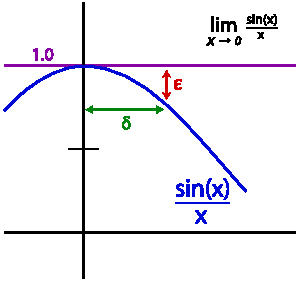
\includegraphics[width=0.90 \linewidth]{epsilondelta.pdf}
\end{center}\vspace{-0.1in}
\caption{ The curvy line is the function $\frac{\sin x}{x}$, which is
  undefined at $0$. However, its limit as $x$ approaches $0$ is $1$.
  The $\epsilon$--$\delta$ formulation of the limit is this: For any
  positive choice of $\epsilon$, there exists some $\delta$ such that
  $\frac{\sin (0 + \delta)}{0 + \delta}$ is less than $1 + \epsilon$.
  In other words, for an arbirarily small error (your choice), I
  can produce a delta from $0$ (my choice) that brings the result
  within the error of the limit. This has nothing to do with the
  subject of the paper.}
\label{fig:epsilondelta}
\end{figure}

\section{Methodology}


Did you know that the SPEC benchmarks~\cite{spec2006} cost \$800? Like
they literally expect me to pay them money to download the source code
so that I could grep for {\tt const double epsilon} or test my
compiler out on that. Mmany are even based on open-source software like
Sphinx and POV-Ray. Ridiculous. I refuse. Values of epsilon for the
SPEC benchmarks do not appear in Figure~\ref{fig:spec}.

\begin{figure}[ht]
\begin{center}

\includegraphics[width=0.99 \linewidth]{spec.pdf}
\end{center}\vspace{-0.1in}
\caption{\$800? Fuck that!}
\label{fig:spec}
\end{figure}



\section{Results}


\begin{figure}[ht]
\begin{center}
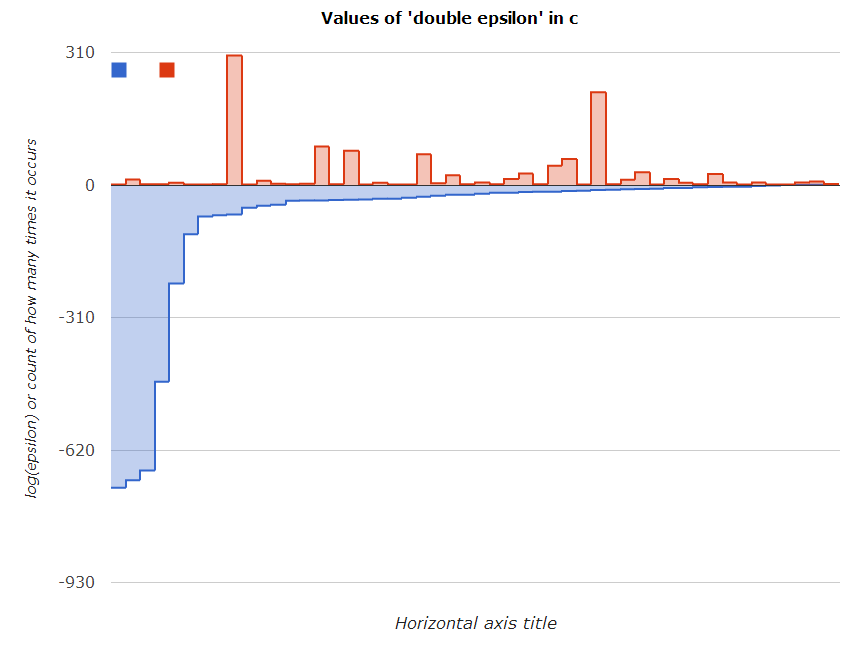
\includegraphics[width=0.99 \linewidth]{chart-c-double}
\end{center}\vspace{-0.1in}
\caption{ Values for {\tt const double epsilon} in the C programming
  language. In this chart, the blue (lower) bars are the distinct values
  of epsilon seen. The vertically aligned red (upper) bar is its count.
  Epsilon values are plotted on a logarithmic scale, where the minimum
  observed value $\log(-708)$ is $303 \times 10^{-308}$, and the largest
  $\log(1.609)$ is $5$. 
  %
  Notes: One programmer used the value \tt{-1e10}, which is
  -10,000,000,000, problably meaning \tt{1e-10}. This value was excluded
  because it has no real logarithm.
}
\label{fig:cdouble}
\end{figure}


\begin{figure}[ht]
\begin{center}
\begin{tabular}{l}
\verb+0.5/ELEC_REST_ENERGY+ \\
\verb+alpha/beta+ \\
\verb+4 / MULT32+ \\
\verb+exact_epsilon(true)+ \\
\verb+fmass_Epsilon * EPS_EXTRA+ \\
\verb+((Lj_Parameters*) parameters)->+ \\
\verb+scalar_traits<+ \\
\verb+EpsArray[prec]+ \\
\verb+hfwfn_->+ \\
\verb+fl.net_.opt_.epsilon+ \\
\verb+Tolerance+ \\
\end{tabular}
\end{center}\vspace{-0.1in}
\caption{ Other uninterpretable values of {\tt const double epsilon}
  in C. Who knows what these are supposed to be?}
\label{fig:cdoubleuninterpretable}
\end{figure}

\begin{figure}[ht]
\begin{center}
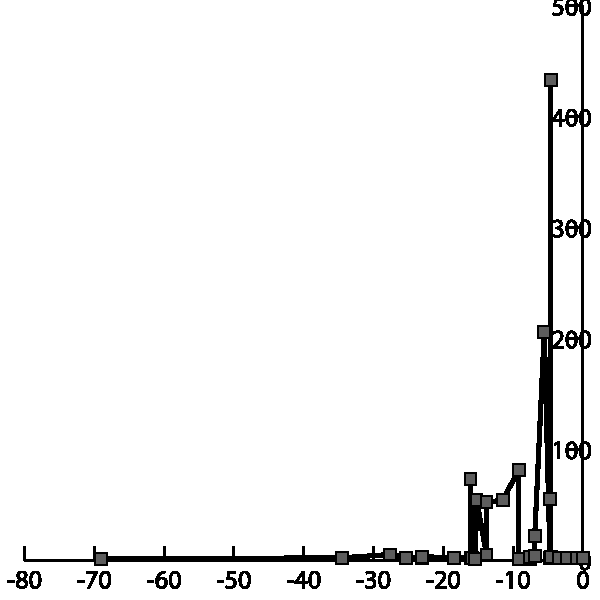
\includegraphics[width=0.99 \linewidth]{chart-c-float}
\end{center}\vspace{-0.1in}
\caption{ Values for {\tt const float epsilon} in the C programming
  language. An $x$--$y$ scatter plot where the $y$ coordinate is the
  count of the number of times that specific value occurred, and the
  $x$ coordinate is the log of the value. Values take on a less
  extreme range than with type {\tt double}, naturally, ranging ``only''
  31 orders of magnitude from $3.9 \times 10^{-31}$ to $0$.}
\label{fig:cfloat}
\end{figure}


\begin{figure}[ht]
\begin{center}
% 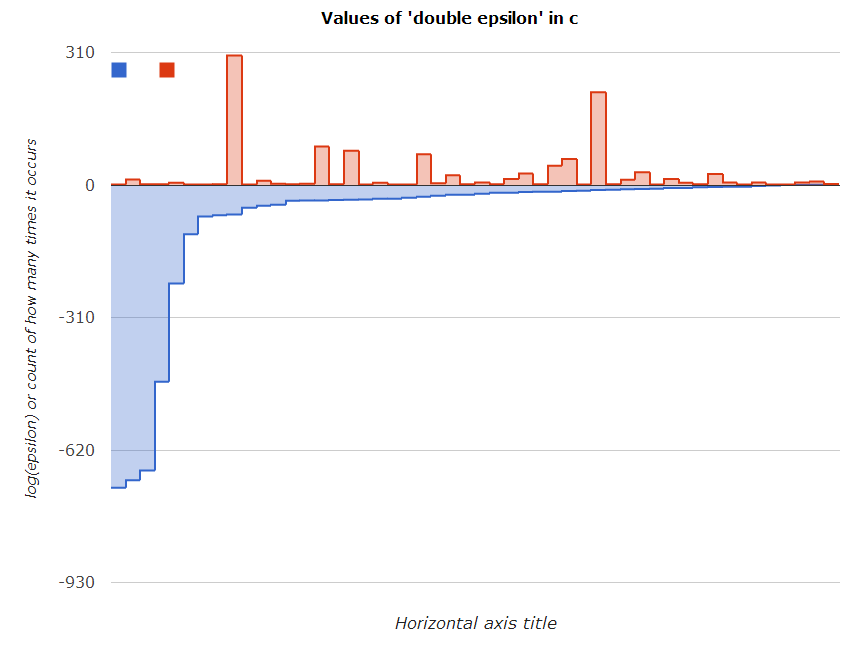
\includegraphics[width=0.99 \linewidth]{chart-c-double}
\end{center}\vspace{-0.1in}
\caption{
  Values for {\tt const double epsilon} and {\tt constexpr
    double epsilon} in the C++ programming language. The {\tt
    constexpr} qualifier, a new feature of C++11, is used very rarely
  (less than 1\% of the time).
  Notes:
  Five times, the computed value is actually equal to 0.0,

  The value {\tt pow(10,-13)} is annotated in German
  ``Genauigkeitsziel bei der Nullstellensuche,'' or ``Accuracy goal in
  the search for zeros.''
}
\label{fig:cppdouble}
\end{figure}


\bibliography{paper}{}
\bibliographystyle{plain}
\end{document}
